% Time-stamp: <2023-09-27 18:49:28 vladimir>
% Copyright (C) 2019-2023 Vladimir G. Ivanović
% Author: Vladimir G. Ivanović <vladimir@acm.org>
% ORCID: https://orcid.org/0000-0002-7802-7970

\begin{comment}
  \section{Charter School Financing}
    \subsection{Charter School Financial Documents}
      \subsubsection{Petitions \& Renewals}
      \subsubsection{Authorizer Staff Reports}
      \subsubsection{Budgets, Interim Reports, and CAFRs}
      \subsubsection{LCAPs,}
      \subsubsection{Board and Committee Supporting Material}
    
  \section{Charter Schools and Real Estate}
    \subsection{Facilities Options}
      \subsubsection{Co-Locating}
      \subsubsection{Leasing}
      \subsubsection{Owning}
    \subsection{Funding Facility Ownership}
      \subsubsection{Private Funding: Loans and Foundation Grants}
      \subsubsection{Venture Funds}
      \subsubsection{Tax Credits}
      \subsubsection{Bonds}
    
  \section{Other Data}
    \subsection{Datasets}
    \subsection{State and Federal Filings}
    \subsection{Curated Social Media}
  
  \section{Gaps and Anomalies}
    \subsection{Triangulation}
\end{comment}

\chapter{Findings}\label{ch:findings}\noindent
This chapter presents data found using the approach outlined in \prettyref{ch:methods} with the goal of answering my research question: ```Has Rocketship structured itself and its finances, to earn a return to investors, focusing especially on real estate transactions, and if so, how?''

The first section presents Rocketship's corporate structure, a structure that separates Rocketship schools from Rocketshhip facilities. The next section, \prettyref{sec:location-and-property-info} details what facilities Rocketship has, where those facilities are located, when they were acquired, and what real estate rights Rocketship has over those properties. Then, given Rocketship real estate, the third section characterizes the finances of Rocketship that are used to fund those properties. \prettyref{sec:equality_equity} looks briefly at issues of fairness. The final section explores what gaps and anomalies were found in Rocketship's financial data.

\section{Rocketship's Corporate Structure}\indent%
\label{sec:RSED-corporate-structure}

Since one of the original four members of Rocketship's board of directors, Eric Resnick, ```provid[ed] a deep
understanding of financial management and real estate transactions'' \parencite{Danner2006}%p.13
, it appears that Rocketship's corporate structure was designed from the start to keep schools and their facilities separate. This structure is diagrammed in \prettyref{fig:corporate-structure} on p. \pageref{fig:corporate-structure}.

\begin{figure}[t]
  \centering\scriptsize
  \caption{\small\emph{Rocketship's Corporate Structure (Santa Clara County facilities only) Schools}}\label{fig:corporate-structure}
  \sffamily
  \begin{forest}
        for tree={grow'=east, folder, draw, align=left}
    [ \textbf{Rocketship Education}, baseline
      [ Launchpad Development Company
        [ \textit{Launchpad (LP)}, xshift=2em ]
        [ \textit{Launchpad Development One LLC (LLC1) RMS facilities}, xshift=2em ]
        [ \textit{Launchpad Development Two LLC (LLC2) RSSP facilities}, xshift=2em ]
        [ \textit{Launchpad Development Threee LLC (LLC3) RLS facilities}, xshift=2em ]
        [ \textit{Launchpad Development Four LLC (LLC4) ROMO facilities}, xshift=2em ]
        [ \textit{Launchpad Development Five LLC (LLC5) RDP facilities}, xshift=2em ]
        [ \textit{Launchpad Development Eight LLC (LLC8) RSA facilities}, xshift=2em ]
        [ \textit{Launchpad Development Ten LLC (LLC10) RSK facilities development}, xshift=2em ]
        [ \textit{Launchpad Development Eleven LLC (LLC11) RBM facilities}, xshift=2em ]
        [ \textit{Launchpad Development Twelve LLC (LLC12) RFZ facilities}, xshift=2em ]
        [ \textit{Launchpad Development Sixteen LLC (LLC16) RRS facilities}, xshift=2em ]
       ]
      [ Rocketship Support Network (RSN) ]
      [ Rocketship Mateo Sheedy Elementary (RSM) ]
      [ Rocketship Sí-Se-Puede Academy (RSSP) ]
      [ Rocketship Los Sue (RLS) ]
      [ Rocketship Mosaic Elementary (ROMO) ]
      [ Rocketship Discovery Prep (RDP) ]
      [ Rocketship Alma Academy (RSA) ]
      [ Rocketship Brilliant Minds (RBM) ]
      [ Rocketship Spark Academy (RSK) ]
      [ Rocketship Fuerza (RFZ) ]
      [ Rocketship Rising Stars (RRS) ]
    ]
    \end{forest}
  \end{figure}

  The parent corporation, Rocketship Education, Inc. (RSED), a 501(3)(c) public benefit corporation, was formed in California on February 16, 2006. RSED owns all the Rocketship schools, Rocketship Support Network, and Launchpad Development Company, a 509(a)(3) nonprofit public benefit corporation.  Launchpad Development Company owns Launchpad and one LLC for each school's facility, generally named ``Launchpad Development <number> LLC''.

  In addition, Rocketship has two entities that are neither schools nor owners of facilities: 
  \begin{itemize}
    \item Rocketship Support Network (RSN) which provides resources for management, back-office support, and organizational strategy
    \item Launchpad (LP) which provides investment and asset management, and administrative services
  \end{itemize}

  This separation between the operation of schools from the funding of their facilities raises the question of why Rocketship has chosen this structure. Some possibilities are:
  \begin{itemize}
    \item Real estate owners are not subject to California's Education Code.
    \item No claims or court actions against the owners of the facilities will extend to the schools themselves.
  \end{itemize}
  
%%%%%%%%%%%%%%%%%%%%%%%%%%%%%%%%%%%%%%%%%%%%%%%%%%%%%%%%%%%%%%%%%%%%%%%%%%%%%%% 
%%% Rocketship Properties
%%%%%%%%%%%%%%%%%%%%%%%%%%%%%%%%%%%%%%%%%%%%%%%%%%%%%%%%%%%%%%%%%%%%%%%%%%%%%%%
  \section{Rocketship Locations and Property Information}\indent%
  \label{sec:location-and-property-info}

  \begin{table}[hbt]
    \caption[Rocketship Property Information]{\textit{Rocketship Property Information}}\label{tab:locations}\SingleSpacing%
    \begin{tabular}{lll}
      \toprule
      School          & Address                               & Property Information \\
      \midrule
      Mateo Sheedy    & 788 Locust St., San José, CA 95110    & \prettyref{sec:mateo-sheedy-info} \\
      Sí Se Puede     & 2249 Dobern Ave, San José, CA 95116   & \prettyref{sec:sí-se-puede-info} \\
      Los Sueños      & 331 S. 34th St, San José, CA 95116    & \prettyref{sec:los-suenos-info} \\
      Discovery Prep  & 370 Wooster Ave, San José, CA 95116   & \prettyref{sec:discover-prep-info} \\
      Mosaic          & 950 Owsley Ave, San José, CA 95122    & \prettyref{sec:mosaic-info} \\
      Brilliant Minds & 2960 Story Rd, San José, CA 95127     & \prettyref{sec:brilliant-minds-info} \\
      Alma Academy    & 198 West Alma Ave, San José, CA 95110 & \prettyref{sec:alma-academy-info} \\
      Spark Academy   & 683 Sylvandale Ave San José, CA 95111 & \prettyref{sec:spark-academy-info} \\
      Fuerza          & 70 S. Jackson Ave, San José, CA 95116 & \prettyref{sec:fuerza-info} \\
      Rising Stars    & 3173 Senter Road, San José, CA 95111  & \prettyref{sec:rising-stars-info} \\
      \bottomrule
    \end{tabular}
  \end{table}

\section{Rocketship's Finances}\indent
\label{sec:rocketship_finances}

  Financing charter schools in California is more complicated than the financing of traditional public schools because charters need to obtain facilities, often independently from the public school district in which they are located.
\prettyref{tab:charter-school-financing-options} describes what facilities financing options a charter school has compared to a traditional public school. Note that ending up with facilities that satisfy a school's needs may require the purchase of land, the construction of new facilities, or the modification of existing facilities in addition to operating those facilities. Each of these alternatives have different potential financing options.

\subsection{Charter School Financing Options}\indent\label{sec:charter-school-financing-options}

\begin{table}[hbt]
  \caption[Charter School Financing Options]{\textit{Charter School Financing Options}}\label{tab:charter-school-financing-options}%
  \SingleSpacing%
  \begin{tabular}{lccl}
    \toprule
    \textbf{Type}        & \multicolumn{2}{c}{\textbf{Available to}}  & \textbf{Notes}\\
                         & \textbf{TSPs} & \textbf{Charters}          & \\
    \midrule
    \multicolumn{4}{l}{State funding} \\
    \midrule
    LCFF                 & Yes  & Yes                        & State minimum guarantee: ADA + adjustments\\ 
    Local property tax   & Yes  & Yes                        & Reduces LCFF amount\\
    Categorical programs & Yes  & Yes                        & \multirow[t]{2}{3in}{All state funding outside of LCFF is\\
                                                               categorical. Some federal programs exist.} \\
    \\
    \midrule
    \multicolumn{4}{l}{Local funding}\\
    \midrule
    Local parcel tax     & Yes  & No                         & Established by district election\\
    Bonds                & Yes  & Yes                        & \multirow[t]{2}{3in}{TSPs: district election; \\
                                                               Charters: private only}\\
    \\
    Construction loans   & Yes  & Yes                        & \multirow[t]{3}{3in}{Typically bonds, with widely varing \\
                                                             terms, but also from the general fund.\\
                                                             Charters: private placement only}\\
    \\\\
    \midrule
    \multicolumn{4}{l}{Federal, state, or private funding}\\
    \midrule
    Private grants       & Yes & Yes                         & Much more common with charters\\
    COVID-19 PPP loans   & No  & Yes                         & Paycheck Protection Program loan \equiv  grant\\
    Venture fund loans   & No  & Yes                         & Often using New Market Tax Credit program\\
    Rent subsidies       & No  & Yes                         & SB740\\
    \bottomrule
  \end{tabular}
\end{table}

The first three sources of financing listed above are considered ordinary revenue and are available to both public schools and to charter schools, although the amounts and timing of the distributions vary. The remainder 

\begin{itemize}
  \item \textbf{LCFF} Local Control Funding Formula. A charter's home district passes through an amount based on a charter's demographics and ADA (Average Daily Attendance). All schools have the same base grant adjusted for grade spans.  If a school has students who are low income (i.e.~they are eligible for free or reduced price meals (FRPM)), or they are English Learners (EL), or they are foster youth, the school receives a supplemental grant of 20\% of its adjusted base grant. If the qualifying population of students exceeds 55\% of the total, a school receives 65\% of the adjusted base grant for every student above the 55\% threshold.

Since all Rocketship schools have at least 55\% of their students , the school qualifies for a LCFF concentration grant in addition to a LCFF supplemental grant. Each qualifying student over the 55\% threshold is entitled to an additional 65\% of the LCFF base grant. Each qualifying student is entitled to an additional 20\% over the base LCFF grant.\\
    \item \textbf{Local property tax} Traditional public school districts are granted the right to tax themselves, using a non-ad valorem tax, by levying a per parcel tax.\footnote{A 2023 court decision allowed a tax based on square footage.}
  \item Local parcel tax] Traditional public school district may assess a non-\textit{ad valorem} tax, usually a per parcel tax. Charter schools do not have taxing authority, so they may not assess parcel taxes.
  \item \textbf{Bonds} Bonds, as far as educational institutions are concerned, come in just a few forms:
        \begin{itemize}
          \item General Obligation (GO) Bonds
          \item Tax and Revenue Anticipation Notes (TRANs) and Revenue Anticipation Notes (RANs)
          \item Conduit Revenue Bonds
        \end{itemize}
  A complete discussion of governmental debt in California is in \textcite{CDIAC2023}.
  
  GO bonds are backed by the full faith and credit of an issuer.  Revenue anticipation notes are backed by specific forms of revenue. Conduit bonds are issued by and are an obligation of a government agency (the conduit) that is neither the borrower nor the purchaser. The government agency is merely a conduit between a borrower and the purchaser(s) of the bond. The conduit borrower's payments to the conduit are sized to meet the payments needed to repay the debt.

  Unlike public school districts that can pass a bond measure based on the value of the entire district's assessed property, charter schools have either no real property (if they are leasing) or a very small amount (if they own their facilities), so even if they were allowed to put a bond measure to the voters, the GO debt limit of 1¼\% of their facilities's assessed value would provide very limited funds. For example, an \$80M valuation would be required to be able to issue a \$1M bond.

  On the other hand, private parties seem to be willing to buy charter school conduit bonds based just on their revenue stream.
 
  \item \textbf{Construction loans}  Construction loans\\
  \item \textbf{COVID-19 PPP} loans COVID-19 PPP loans\\
  \item \textbf{Venture fund loans} Venture fund loans\\
  \item \textbf{Private grants} Private grants\\
  \item \textbf{Rent subsidies} Rent subsidies\\
\end{itemize}

\subsection{Rocketship Financial Documents}\label{sec:rocketship-financial-docs}\indent

Every year, as required by law, Rocketship issues an independently audited financial statement for the preceeding school year. Rocketship, rather than issuing a separate financial statement for each of its affiliates, consolidates them into a single document, typically titled \emph{Rocketship Education, Inc. and Its Affiliates Consolidated Financial Statements and Supplementary Information Year Ended June 30, xxxx}. Four annual financial statements are reported:

\begin{itemize}
  \item Financial Position, which corresponds to a business's balance sheet\\
  \item Activities, which corresponds to a business's income statement\\
  \item Cash Flows, which corresponds to a business's cash flow statement\\
  \item Functional Expenses, which has no corresponding business statement\\
\end{itemize}

Each annual financial statement, starting with the YE 2011, includes a disclaimer such as, ``All significant intercompany accounts and transactions within RSED and its schools have been eliminated in the consolidating financial statements.'' Although this may be standard accounting practice, it does make getting a complete picture of Rocketship's finances harder because some transactions effectively disappear from the consolidated statements. Elminated transactions are nonetheless recorded and   

The four different financial statements for the years 2010–2022\footnote{The years ending 2008 (2007–2008) and 2009 (2008-2009) have not been included in some summaries because they were different from all the other years. The year 2009 included 2008, and 2008 was restated in 2022.} were collected and the data summarized. These summaries appear in \prettyref{tab:consolidated_financial_position}, \prettyref{tab:consolidated_activities}, \prettyref{tab:consolidated_cash_flows}, and \prettyref{tab:consolidated_functional_expenses}, and online in this dissertation's \textit{Data Dashboard}, a Google spreadsheet.%
\footnote{\url{https://docs.google.com/spreadsheets/d/1c4akEKFj9bmVfLFQwi7ewMifSjRbrw5xpjh_UjO4oYY/edit?usp=sharing}}

Rocketship's net assets from 2010 to 2022 have always been positive.
\begin{table}[ht]\caption{Net Assets, 2010–2022}\label{tab:net_assets}
  \begin{tabular}{lll}
    \toprule
    \textbf{Year} & \textbf{Net Assets} & \textbf{Annual Increase}\\
    \midrule
    2010 &   \$2,218,964	&            \\
    2011 &   \$9,212,140	&   315.16\% \\
    2012 &  \$11,933,099	&    29.54\% \\
    2013 &  \$15,881,210	&    33.09\% \\ 
    2014 &  \$13,356,528	&   -15.90\% \\
    2015 &  \$10,562,747	&   -20.92\% \\
    2016 &  \$16,931,464	&    60.29\% \\
    2017 &  \$17,536,163	&     3.57\% \\
    2018 &  \$20,883,606	&    19.09\% \\
    2019 &     \$187,450        &   -99.10\% \\
    2020 &  \$24,617,294        & 13032.73\% \\
    2021 &  \$38,231,318	&    55.30\% \\ 
    2022 &  \$33,442,645        &   -12.53\% \\
    \bottomrule
  \end{tabular}
\end{table}


\begin{figure}[t]
  \centering
  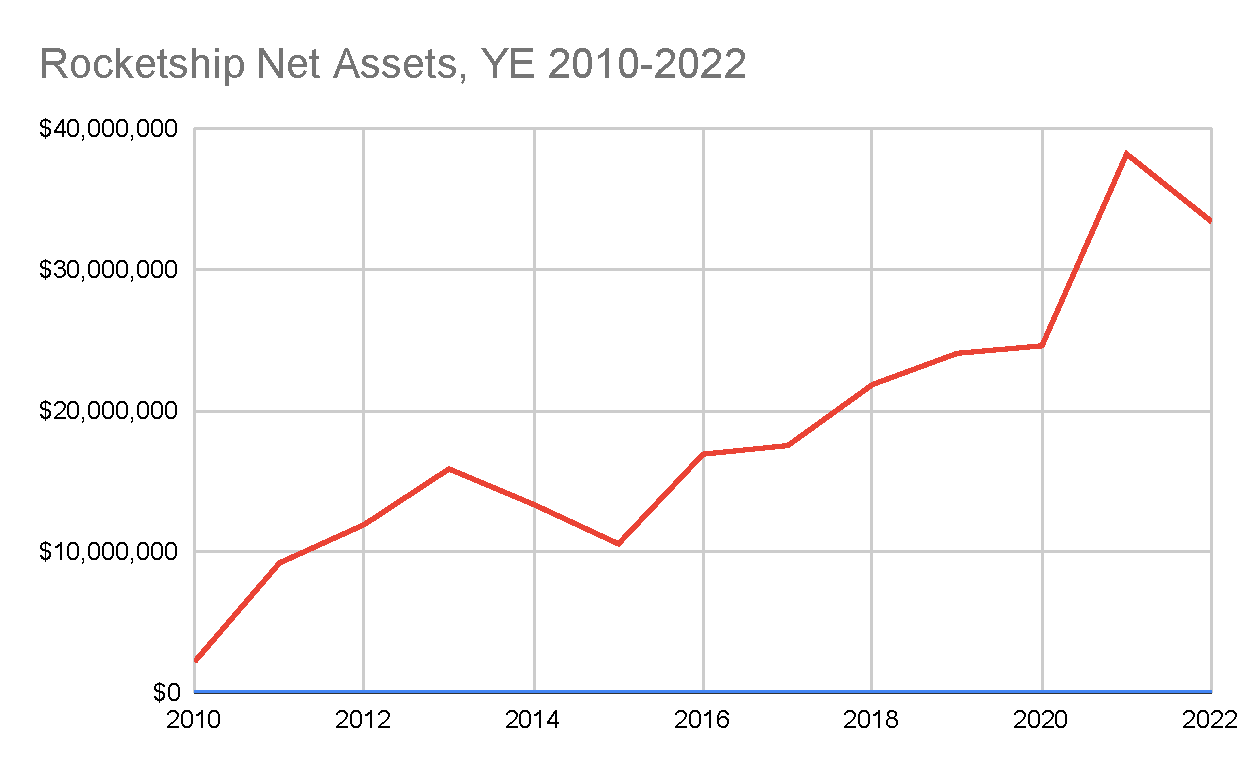
\includegraphics[width=\textwidth,keepaspectratio]{Net_Assets}%
  \caption{Rocketship Net Assets, YE 2010-2022}%
  \label{fig:net_assets}
\end{figure}

\begin{figure}[b]
  \centering
  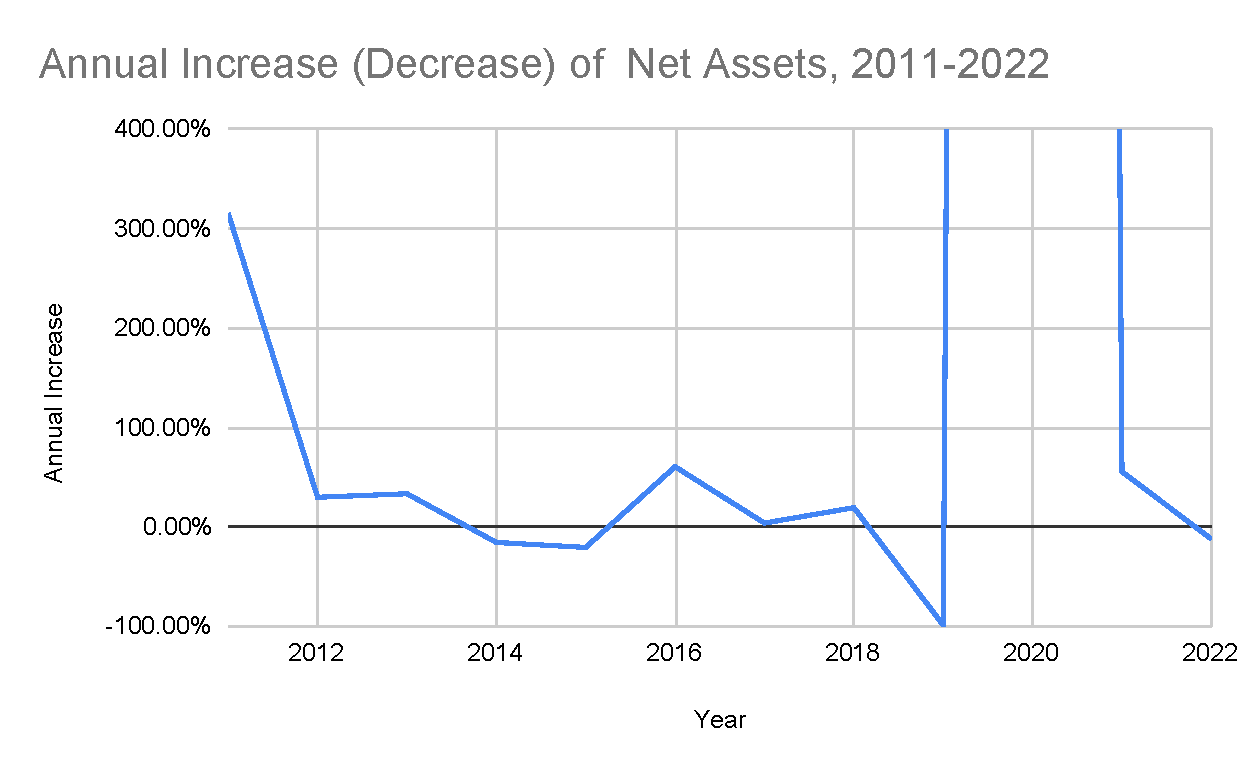
\includegraphics[width=\textwidth,keepaspectratio]{Annual_Increase_Net_Assets_2011-2022}%
  \caption{Annual Increase in Net Assets, 2011-2022}%
  \label{fig:annual_net_asset_increases}
\end{figure}


% \subsubsection{Financial Position}\indent%
% \label{sec:financial_position}

% \subsubsection{Activities}\indent%
% \label{sec:activities}

% \subsubsection{Cash Flows}\indent%
% \label{sec:cash_flows}

% \subsubsection{Functional Expenses}\indent%
% \label{sec:functional_expenses}

\subsection{Debt}\indent%
\label{sec:debt}

Rocketship has borrowed over 50 times since its founding in 2006\footnote{Full details of Rocketship's borrowings are in this dissertation's Google spreadsheet (see the previous footnote) in the tab \textit{Dashboard} starting on lines 10–63.} 
and their annual, consolidated financial statements provide debt summaries starting in 2012. The totals are shown in \prettyref{tab:total_debt} and in \prettyref{fig:total_debt} on p.\pageref{fig:total_debt}.

The annual increase (or decrease) in debt year over year is shown in \prettyref{fig:annual_debt_increases} on p.\pageref{fig:annual_debt_increases}. One can immediately make two observations:
\begin{enumerate}
  \item The swings are quite pronounced, ranging from nearly a 60\% in 2014 to two lows of \approx 15\% decreases in 2015 and in 2022.
  \item The overall trends seems to be a gradual decline, perhaps reaching 0\% in 2023 or 2024.
\end{enumerate}

\begin{table}[ht]\caption{Total Debt, 2012-2022}\label{tab:total_debt}
  \begin{tabular}{lll}
    \toprule
    \textbf{Year} & \textbf{Total Debt} & \textbf{Annual Increase}\\
    \midrule
    2012 &  \$47,046,048 & \\
    2013 &  \$57,078,166 & 121.32\% \\
    2014 &  \$88,383,082 & 154.85\% \\
    2015 &  \$75,904,098 &  85.88\% \\
    2016 & \$104,857,696 & 138.14\% \\
    2017 & \$136,652,562 & 130.32\% \\
    2018 & \$129,391,897 &  94.69\% \\
    2019 & \$163,598,844 & 126.44\% \\
    2020 & \$168,701,124 & 103.12\% \\ 
    2021 & \$196,416,045 & 116.43\% \\
    2022 & \$186,550,566 &  85.89\% \\
    \bottomrule
  \end{tabular}
\end{table}

\begin{figure}[t]
  \centering
  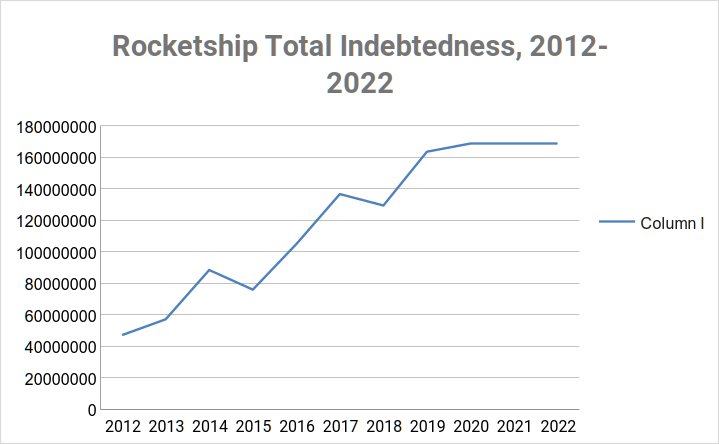
\includegraphics[width=\textwidth,keepaspectratio]{Debt}%
  \caption{Rocketship Indebtedness, 2012-2022}%
  \label{fig:total_debt}
\end{figure}

\begin{figure}[b]
  \centering
  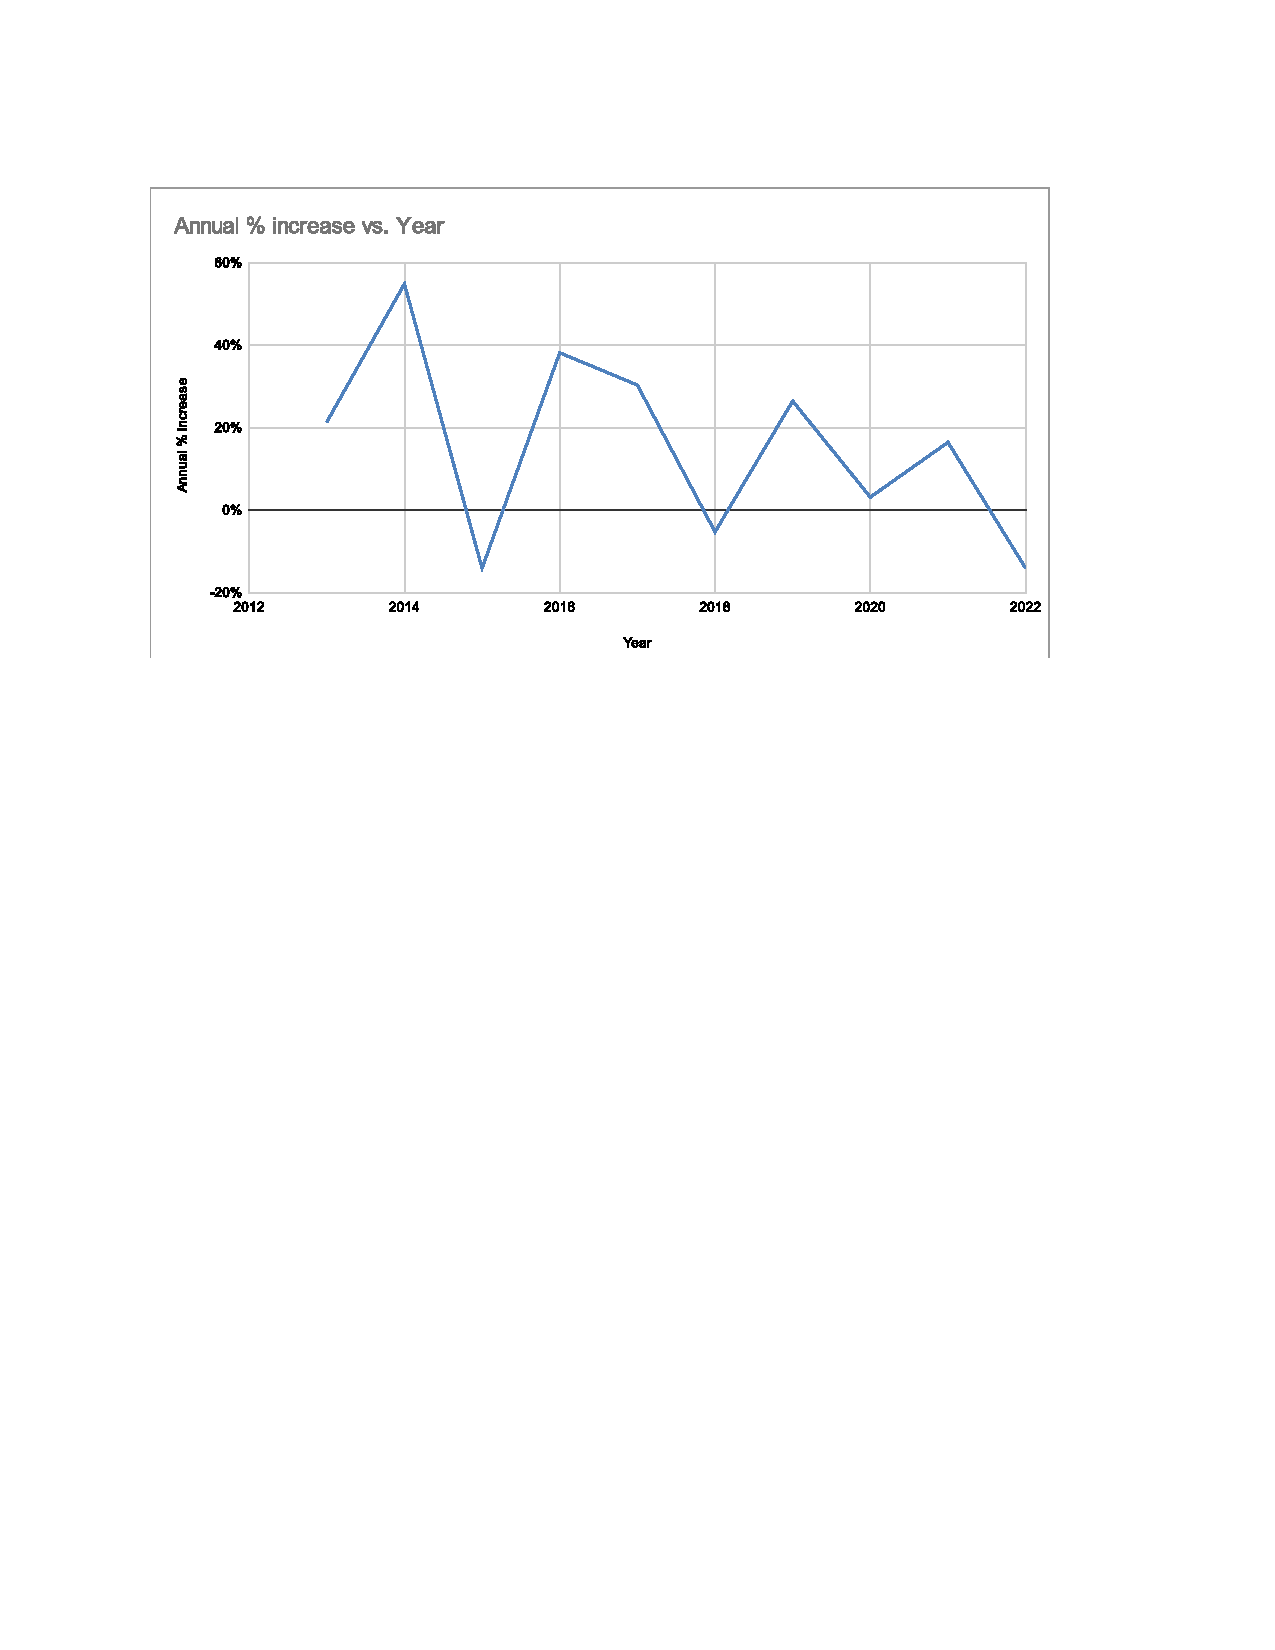
\includegraphics[width=\textwidth,keepaspectratio]{Annual_Debt_Increases}%
  \caption{Rocketship Indebtedness, 2012-2022}%
  \label{fig:annual_debt_increases}
\end{figure}

\subsubsection{Debt Summary}\indent%
\label{sec:debt_summary}

\subsubsection{Financing Debt}\indent%
\label{sec:financing_debt}

\paragraph{Letters of Credit}
\paragraph{Municipal Bonds}
\paragraph{Conduit Bonds}

\subsection{Non-Debt Financing}\indent%
\label{sec:non_debt_financing}

\subsubsection{Donations and Grants}\indent%
\label{sec:donations_grants}

\subsubsection{Forgiveness of Debt}\indent%
\label{sec:forgiveness_debt}

\subsubsection{Loans}\indent%
\label{sec:loans}

\subsubsection{Venture Funds}\indent%
\label{sec:venture_funds}

\subsection{Tax Credits}\indent%
\label{sec:tax-credit}

The New Market Tax credit of 39\% (5\% for the first 3 years, and 6\% for the remaining 4 years) can be applied to taxes due from other investments. Since there is a compounding effect, the 39\% is actually worth over 41\% of the initial investment. Note that these other investment may themselves have a return. With these kinds of incentives, it's no wonder that the New Markets Tax Credit is popular. But one should not be deceived into thinking that just because New Markets Tax Credits must be made in economically depressed area that investors are investing out of the goodness of their heart. The tax credit investment is nearly without risk because the tax credit is guaranteed as long as the charter school remains open. If the school stays open for seven years, the risk is zero.

\subsection{Equality and Equity}\indent%
\label{sec:equality_equity}

\subsubsection{Location and Concentration Grants}\indent%
\label{sec:tax-credit}

\subsubsection{Student Instruction and Support}\indent%
\label{student_instruction_support}

\section{Gaps and Anomalies}\indent%
\label{sec:findings-gaps-anomolies}

% \subsection{Real Estate Data}\label{sec:real-estate-data}\indent
% \begin{enumerate}
%   \item What is the actual price, date, and buyer \& seller information for each property?
%   \item What is the legal relationship between Rocketship Education and Launchpad Development?
%   \item How were Rocketship facilities in Santa Clara County financed?
%   \item What are the type and terms of all bonds.
%   \begin{enumerate}
%     \item What bonds were floated: type, rate, \& terms; guaranteed by whom or how? If the bonds are not privatedly placed, they are classed as securities, and their prospectuses are filed with the Securities Exchange Commission and are publicly viewable.
%     \item For conduit bonds, the California Department of Education or Department of Finance web sites 
%   \end{enumerate}
%   \item Enumerate all known leases and their terms. Was part of the lease payment paid by California?
%   \item Enumerate all known loans.
%   \begin{enumerate}[a.]
%     \item What was used as collateral? 
%     \item What were the terms?
%   \end{enumerate}    
%   \item Enumerate donations from foundations and individuals.
%   \item Enumerate venture fund investments.
% \end{enumerate}


% Forms which have been filed with a government entity:
%  \begin{enumerate}
%   \item Federal 990 forms to check against financial statements. IRS maintained. Should cross-reference the financial statements.
%   \item Annual and interim budgets submitted to the California Department of Education.
%   \item Petition approvals and renewals submitted to local school districts, the SCCOE, or the California State Board of Education.

%   The Santa Clara County Office of Education (SCCOE), and each school district in which Rocketship petitioned to open a school has some data/notes from one or more board meetings in which the petition or renewal was discussed. These data might have been presented by Rocketship or by county or district staff. Sometimes there is also public comment.
  
% Often, petitions presented to a school district have been denied and appealed to the Santa Clara County Board of Education, and in a few cases, to California's State Board of Education.
  
%   \item There is some published material on Rocketship.
%   \begin{enumerate}[a.]
%     \item Some books have been written about Rocketship
%     \item Roxana has two ScoopIt collections on Rocketship on and charter schools.
%     \item The ``Stop Rocketship'' web site has lots of information on Rocketship.
%     \item Several academics have datasets of school or district financial information  which include Rocketship.
%     \item Numerous articles, web sites, and blog postings include Rocketship financial data.
%   \end{enumerate}
%   \item Other, outside entities that may add revenue to Rocketship
%   \begin{enumerate}
%     \item Zeal
%     \item Dreambox Learning
%   \end{enumerate}
% \end{enumerate}

 

% Since a goal of this dissertation is to map the flow of money into and out of Rocketship, I will use diagrams similar to the one used by \citeauthor{Baker.Miron2015} (\citeyear{Baker.Miron2015}), which is reproduced here as \prettyref{fig:opresflows}.

% \subsection{Triangulation}\label{sec:findings-triangulation}\indent

% These data represent the monies that are flowing into Rocketship/Launchpad related to facilities, real estate, bonds, loans, and donations and not tied to the number of students. Once that's been assembled, roll up into one spreadsheet, Rocketship's consolidated financial statements for the fourteen years (2008--2022). The consolidated financial statements can then be compared against the known real estate, bond, loan, and donation transactions. Noe where data is missing or where it conflicts with the consolidated financial statements.

% \begin{figure}[ht]
%   \centering
%   \caption[Operating Resource Flows]{\textit{Operating Resource Flows}}\label{fig:opresflows}
%   \includegraphics[width=\textwidth]{Operating_Resource_Flows}\\
%   \footnotesize\raggedright\textcite[16]{Baker.Miron2015}.
% \end{figure}
% In this example, money flows from left to right, and there are no loops. Colors are used merely to distinguish the various blocks.

%%% Local Variables:
%%% mode: latex
%%% TeX-master: "Rocketship_Education-An_Exploratory_Public_Policy_Case_Study"
%%% End:
